\documentclass[11pt]{article}

\usepackage[utf8]{inputenc}
\usepackage[T1]{fontenc}
\usepackage[french]{babel}
\usepackage{cite}
\usepackage{amssymb}
\usepackage{amsmath}
\usepackage{mathrsfs}
\usepackage{graphicx}

\title{Projet Robotique Autonome\\
\textit{Robot Humanoïde Sigmaban : optimisation de la marche}}
\author{Maxime Carrere, Quentin Maouhoub, Quentin Rouxel}
\date{31/01/2013}

\begin{document}

\maketitle

\section{Introduction}

L'objet de ce projet est l'optimisation de la marche du robot de l'équipe 
de recherche Rhoban : Sigmaban. Il s'agit d'un robot humanoïde possédant deux bras,
deux jambes, et composé d'un total de 20 servomoteurs. La finalité de ce projet est de faire
participer Sigmaban à la RoboCup 2013.

\section{Mise en place de l'environnement}

Les servomoteurs articulant le robot sont tous connectés en série sur un même 
bus. Le protocole utilisé pour communiquer au travers de ce bus série est défini par le
constructeur des servomoteurs \textit{Dynamixel}. Le bus série est ensuite relié à un mini pc
embarqué sur le robot par connexion USB. Ce mini pc fait tourner un environnement linux
(distribution debian) sur lequel est installé \textit{Rhoban Server}, qui assure la communication
bas niveau avec les servomoteurs ainsi que l'ordonnancement des différents mouvements. Le mini pc
a été configuré pour rejoindre un point d'accès WiFi. Il est ainsi possible de contrôler le robot
à distance.

\section{Stabilisation et premiers mouvements}

La création des primitives motrices est réalisée à l'aide de l'interface graphique de Rhoban.
Elle permet, à l'aide d'un système de blocs interconnectés,
de construire facilement le signal à appliquer aux actionneurs du robot. Les mouvements ainsi générés
sont ensuite transmis au serveur embarqué sur le robot qui se charge de les exécuter.\\

La première étape est le système d'équilibrage du robot. Les articulations des pieds, des genoux 
et des hanches sont utilisées pour contre-balancer les chocs et déséquilibres permanents
du robot. Ce dernier dispose de capteurs accéléromètres et gyroscopes selon des axes frontaux et sagittaux.
A partir de ces capteurs, des boucles de régulation proportionnelles et proportionnelles intégrales appliquées
aux articulations permettent de maintenir debout le robot.\\

Les mouvements sont ensuite créés, basés sur un signal sinusoïdal. Le gain et la phase du signal périodique 
sont éventuellement modifiés puis envoyés aux différentes articulations. Ces entrées sinusoïdales constituent l'ensemble des paramètres du mouvement que la méthode d'apprentissage pourra faire varier. Le mouvement réalisé fait piétiner le robot 
toujours debout en déplaçant sont poids d'un pied sur l'autre.

\section{Détermination d'une fonction récompense}
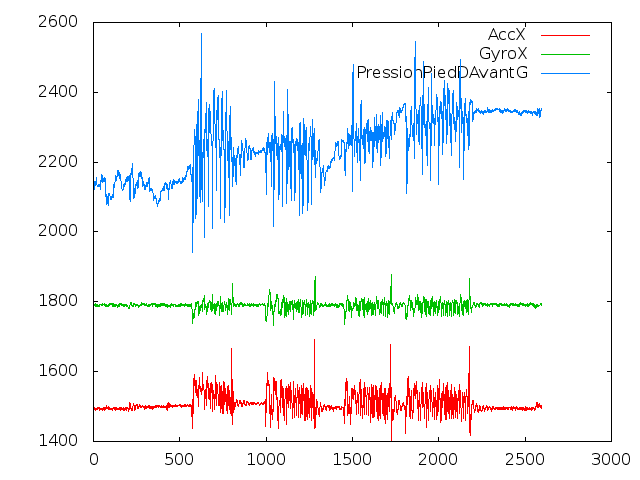
\includegraphics[scale=0.4]{sensors.png}
Afin de mettre en place un apprentissage, il fallait que le robot puisse évaluer à chaque essai la qualité de sa marche. Ainsi, en cherchant à maximiser cette qualité, le robot va, petit à petit, se déplacer de façon plus efficace.\\
Dans le cas présent, la fonction attribuant une note à la marche, ou fonction de récompense, prend en paramètre les relevés des différents capteurs de SigmaBan: 4 capteurs de pression sous chacun de ses pieds, deux accéléromètres mesurant l'inclinaison du robot par rapport au plan de déplacement, un capteur d'élongation à chaque hanche, mesurant l'inclinaison du buste par rapport au bassin, et finalement deux gyroscopes en X et Y, pour mesurer les accélérations. Les positions des différents moteurs de sigmaban ne sont donc pas prises en compte pour noter la qualité de la marche.\\
La fonction de récompense prend en entrée les relevés de ces capteurs tout au long d'une phase de marche, et donne en sortie une unique valeur, mesurant la qualité de cette phase de marche. Le problème qui se posait donc était de parvenir à rassembler ces mesures diverses et variées en une seule valeur. Nous sommes partis de l'hypothèse qu'une bonne mesure de la marche est sa périodicité, une bonne marche se répétant à l'infini, et étant donc parfaitement périodique.\\
Notre fonction de récompense fonctionne en trois temps:
\begin{itemize}
\item En premier lieu, elle utilise l'ensemble des relevés pour déterminer les phases de marche du robot. En effet les enregistrements effectués possèdent des périodes de marche entrecoupées de périodes où le robot est au repos. Nous normalisons l'ensemble des valeurs fournies par les capteurs, puis nous calculons la somme de ces valeurs à chaque instant. Les périodes de marche ressortent alors clairement, car les valeurs obtenues par les différents capteurs sont pour la plupart plus importantes lors du déplacement. De plus sommer ainsi les différentes valeurs des capteurs permet de préciser les périodes, en éliminant les faux positifs quand l'un des capteurs est defectueux (dans notre cas l'un des capteurs de pression des pieds).
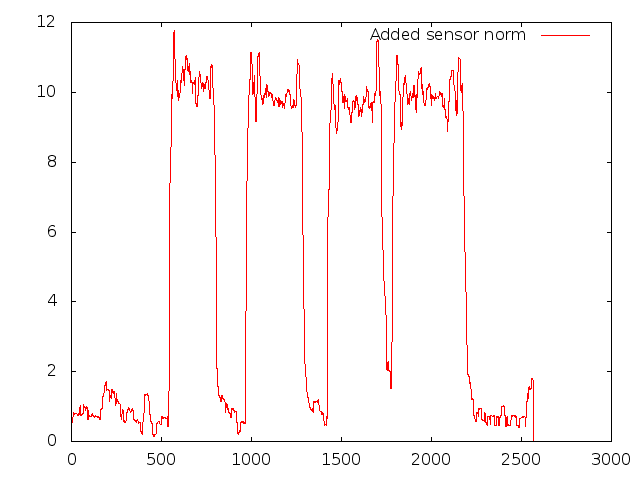
\includegraphics[scale=0.4]{walks.png}
\item Dans un second temps, nous effectuons pour chaque capteur la transformée de Fourier des relevés, ce qui nous permet d'obtenir l'harmonique principale (le mouvement imprimés aux moteurs étant effectivement sinusoidal). En calculant la phase de cette harmonique, nous pouvons ainsi distinguer les périodes du mouvement pour chaque capteur.
\item Ces périodes nous permettent de positionner chaque valeur échantillonnée dans le mouvement (savoir où se trouve se point dans la période du mouvement en cours). En calculant la variance entre points correspondants de différents périodes (ces points sont situés aux mêmes endroits dans différentes périodes, et devraient donc avoir la même valeur si le mouvement était parfaitement périodique), nous obtenons une mesure de la périodicité du mouvement. 
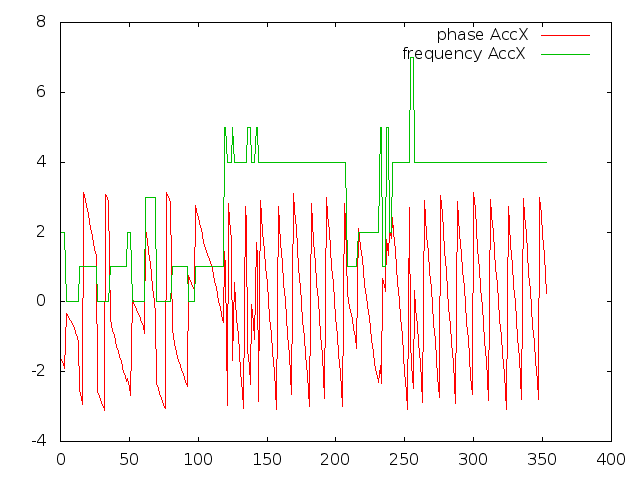
\includegraphics[scale=0.4]{phase_freq.png}
\end{itemize}
En sommant ces variances pour les différents capteurs,
nous obtenons donc une valeur qui mesure la périodicité globale d'un mouvement. Plus cette valeur est petite, plus le mouvement est périodique, et donc plus le robot doit privilégier les paramètres correspondants aux mesures pour optimiser sa marche. 
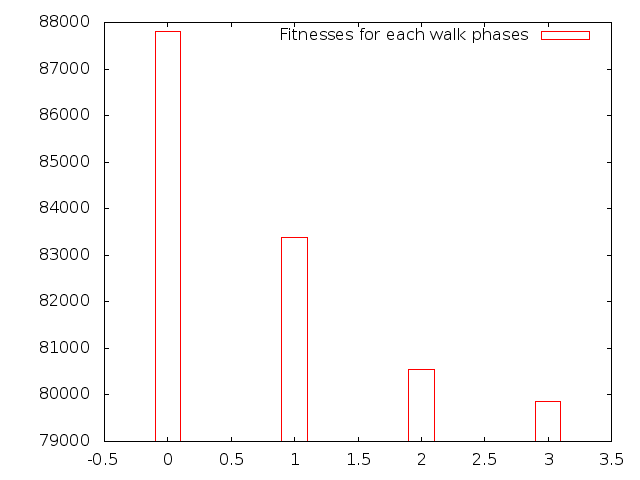
\includegraphics[scale=0.4]{fitnesses.png}
\section{Optimisation de la marche}
\subsection{Exploration locale}
Grâce à la fonction de récompense précédemment présentée, on peut déterminer des paramètres pour lesquels le robot marche "mieux" que d'autres. Avec un ensemble de n listes de p paramètres, chacune associée à un score, on peut donc sélectionner un certain nombre l de ces listes, celles avec le  meilleur score. A partir d'une des listes sélectionnées, il est possible d'explorer localement autour du point qu'elle définit dans un espace à p dimensions. On génère donc pour chacune des listes sélectionnées, un certain nombre de listes proches dans cet espace, c'est-à-dire dont les valeurs des paramètres sont proches des valeurs des paramètres correspondant dans la liste originelle.\\
On obtient donc un nouvelle ensemble de $n_2$ listes de p paramètres, comprenant la meilleure de l'ensemble précédent et les nouvelles listes générés à partir de celles-ci. On peut donc espérer que notre nouvel ensemble possède des listes de paramètres mieux notées que le précédent. Il faut cependant calculer le score obtenu par chacune des listes nouvellement créées, en fournissant ces listes l'une aprés l'autre en entrée du robot, et analyser les différents résultats fournis par les capteur du robot lors de l'éxécution du mouvement. On va donc ainsi améliorer petit à petit les résulats obtenus par les listes de paramètres, de manière à trouver les maximums locaux de la fonction de récompense.

\subsection*{Exemple} 
On part avec 5 listes de 3 paramètres entiers, chaque liste ayant un score entier associé:\\
L1=\{0;12;45\}; L1\_Score=154;\\
L2=\{3;1;5\}; L2\_Score=102;\\
L3=\{40;67;12\}; 
L3\_Score=87;\\
L4=\{73;24;7\};  
L4\_Score=167;\\
L5=\{23;17;64\}; 
L5\_Score=17;\\

On sélectionne les 2 meilleures listes, L4 et L1, et on génère à partir de chacune d'elles deux listes nouvelles, en faisant en sorte que les paramètres soient proches à 10\% près. On obtient ainsi 5 listes de 3 paramètres :\\

L1=\{73;24;7\}
L2=\{67;22;7\}
L3=\{75;25;7\}
L4=\{0;13;42\}
L5=\{0;12;44\}

Pour calculer les scores associées à chacune des listes de paramètres, on doit passer ceux-ci au robot, et générer la valeur du score grâce aux différentes données fournies par les capteurs. Nous pouvons également changer le nombre de liste à garder, et donc le nombre de copies à générer.

\section{Conclusion}
Nous avons ainsi pu installer les outils fournis par Rhoban sur Sigmaban, pour communiquer avec lui et lui donner des ordres, et avons implémenté un modèle de calcul pour son apprentissage de la marche. Cependant, nous n'avons pas pu tester sur Sigmaban l'efficacité de notre système. D'une façon générale, il y avait de nombreuses pistes que nous aurions aimé explorer, comme prendre en compte l'amplitude du mouvement et -de façon négative- les autres harmoniques, pour obtenir une fonction de fitness plus robuste. Au niveau des paramètres d'entrée, normaliser les valeurs des capteurs dans RhobanServer avant toute série de mesure permettrait d'avoir des valeurs cohérentes entre deux sessions. 
\section{Remerciements}
Nous remercions Grégoire Passault pour avoir fortement contribué à l'obtention des résultats de marche de Sigmaban.

\section{Annexes}
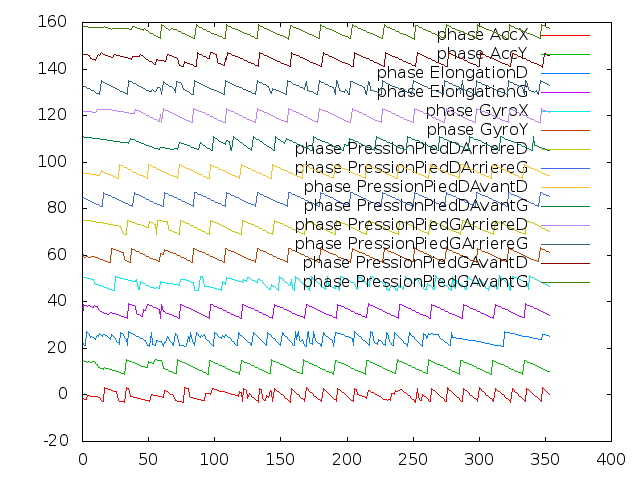
\includegraphics[scale=0.4]{all_sensor_phases.png}
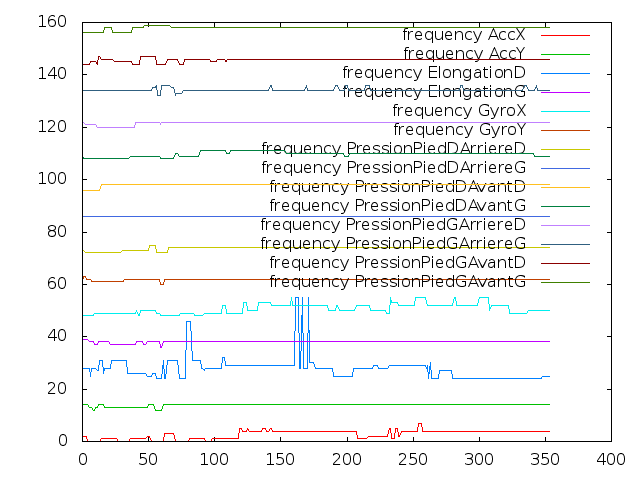
\includegraphics[scale=0.4]{all_sensor_freq.png}

\end{document}

